
\section{Background and Related Work}
\label{sec:backgr-relat-work}


\subsection{The MiGen System}
\label{sec:migen-system}

The MiGen system supports classes of students in undertaking algebraic
generalisation tasks using a mathematical microworld called the 
{\bf eXpresser}. Using the eXpresser, students are asked to construct
two-dimensional tiled patterns, which may be painted in different
colours, and to derive general rules for the number of tiles of each
colour required to paint each pattern and their model
overall. Students are prompted to create `building-blocks' to
construct their patterns, depending on their perceptions of the
pattern’s structure. Each building block is made up of a group of
tiles, and can be repeated horizontally, vertically or diagonally to
contribute to the construction of the pattern. For example, Figure 1
shows an example model that students may be asked to construct. They
will be nudged by the system towards creating building-blocks to
generate the centres of the flowers, the petals, and the stalks, and
towards deriving rules for the number of red tiles and the number of
green tiles required to paint the model, given the number of yellow
tiles.

\begin{figure}[htbp]
  \centering
  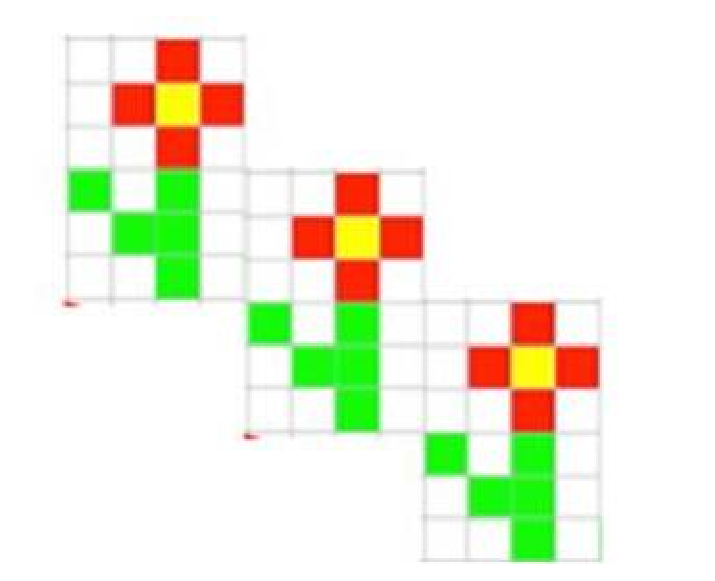
\includegraphics[width=6cm]{gfx/example.eps}
  \caption{An example model that students may be asked to construct in eXpresser}
  \label{fig:example}
\end{figure}



%%% Local Variables:
%%% mode: latex
%%% TeX-master: "main"
%%% End:
